\subsection{Problem A3} Denote the real numbers as $\R$ and the complex numbers as $\C$. Example of a limit:

    \begin{equation}
        z = \lim_{s\to0^+}\frac{s+1}{s^3+s^2-5s+9}.
    \end{equation}
    
    Another example
    \begin{equation}
        \lim_{s\to\infty} \frac{s+1}{s^3+s^2-5s+9}.
    \end{equation}
    
    Example of an integral
    \begin{equation}
        \int_0^\infty e^{-s\tau}f(\tau)\dd\tau.
    \end{equation}
    
    Three aligned equations
    \begin{align}
        a =& 1,
        \\
        b =& 2,
        \\
        c =& 3.
    \end{align}
    
    Two aligned equations without equation numbers
    \begin{align*}
        a =& 1,
        \\
        b =& 2.
    \end{align*}
    
    Mathematical derivations aligned at the ``='' sign:
    \begin{align}
        \frac{1}{2+3j} {}={}& \frac{2-3j}{(2+3j)(2-3j)}
        \notag\\
        {}={}& \frac{2-3j}{2^2 + 3^2}
        \notag\\
        {}={}& \frac{2-3j}{13}
        \notag\\
        {}={}&\frac{2}{13} - j\frac{3}{13}.
    \end{align}
    
    More mathematical derivations:
    \begin{align*}
        & as + 4 + 2s = b + (8+a)s
        \\
        \Leftrightarrow{}& (a+2)s + 4 = b + (8+a)s
        \\
        \Leftrightarrow{}& (a+2)s - (8+a)s = b - 4.
    \end{align*}
    
    Boldface math: $\bm{x}$. Vectors:
    \begin{equation}
        \bm{x} = 
        \begin{bmatrix}
            x_1
            \\
            x_2
            \\
            x_3
        \end{bmatrix}.
    \end{equation}
    
    Another example: According to Taylor's Theorem:
    \begin{equation}
        \phi(x) \approx \phi(x_0) + \phi'(x_0)(x-x_0).
    \end{equation}
    
    Partial derivatives:
    \begin{equation}
        \label{eq:partial_derivatives}
        \frac{\partial f(x, y)}{\partial x} = x^2\cos(xy).
    \end{equation}
    
    \begin{tcolorbox}[title={Common typesetting mistakes}]
        \textbf{Important Note:} 
        \begin{itemize}
            \item Write $\cos x$, not $cos x$.
            \item Write $\sin x$, $\log x$, etc --- not $sin x$, $log x$ and so on.
            \item Write $\lim_{s\to 0^+} sF(s)$, not $lim_{s\to 0^+} sF(s)$.
            \item Write $F(s)$, not $F(S)$. 
            \item Write $xy$, or $x\dot y$, but not $x*y$ --- that would be the \textit{convolution} of     $x$ with $y$, not their product, so
                \begin{equation}
                    2 * 3 = 3t^2.
                \end{equation}
            \item To denote a variable with a subscript, write $x_1$, not $x1$.
            \item For superscripts, write $x^2$, not $x2$.
            \item Denote a variable by $x$, not x. 
            \item Double quotes are ``like this'', not "like this".
            \item Reference equations using: Equation \eqref{eq:partial_derivatives}; not Equation \ref{eq:partial_derivatives} and not Equation (12).
        \end{itemize}
    \end{tcolorbox}
    
    
    
    % You can write comments like this
    \begin{figure}[h]
        \centering
        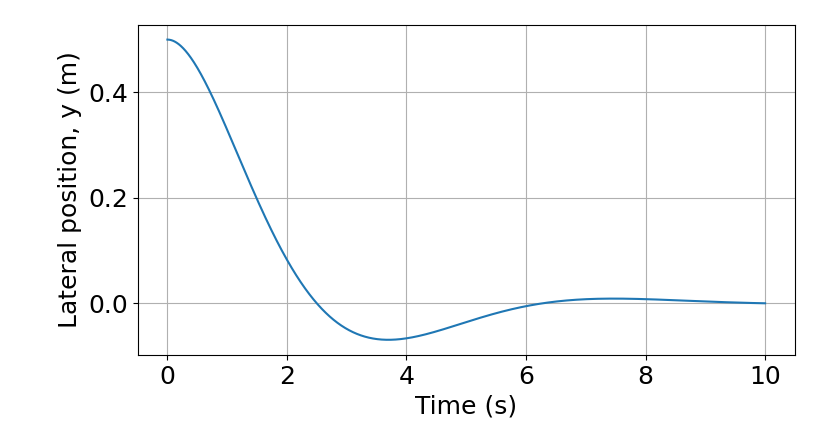
\includegraphics[width=0.65\linewidth]{figures/lateral_position}
        \caption{You may of course include figures in your document. Make sure your figures have legible axis labels. Figures of about this size are perfectly legible.}
    \end{figure}
